\documentclass{article}

\usepackage[main=english,vietnamese]{babel}
\usepackage[T1]{fontenc}
\usepackage[utf8]{inputenc}
\usepackage[sexy]{evan}
\usepackage{matchsticks}
\usepackage{wrapfig}
\usepackage{listings}

\begin{otherlanguage*}{vietnamese}
\title{Các kỳ thi Toán Canada: Nền tảng nuôi dưỡng những tài năng toán học trẻ}
\end{otherlanguage*}

\author{Nghia Doan}
\date{\today}

\begin{document}

\begin{otherlanguage*}{vietnamese}

\maketitle

\textbf{Giới thiệu về các kỳ thi toán Canada (Canadian Mathematical Competition - CMC)}

Các kỳ thi toán Canada là một loạt các cuộc thi được tổ chức bởi Hội Toán học Canada (Canadian Mathematical Society - CMS)
nhằm khuyến khích và phát triển niềm đam mê toán học cho học sinh từ nhiều lứa tuổi, đặc biệt là học sinh trung học.
Các cuộc thi không chỉ là một sân chơi trí tuệ, mà còn là một nền tảng để phát triển kỹ năng tư duy logic,
khả năng giải quyết vấn đề và sự sáng tạo toán học của học sinh.

CMS đã tổ chức nhiều cuộc thi toán học khác nhau, bao gồm các kỳ thi dành cho học sinh trung học cơ sở, trung học phổ thông và các kỳ thi mở dành cho mọi học sinh muốn thử thách bản thân.
Cùng với mục tiêu tuyển chọn và phát hiện những tài năng toán học cho các cuộc thi quốc tế,
CMC đã góp phần thúc đẩy giáo dục toán học tại Canada, tạo ra một cộng đồng học sinh yêu thích và đam mê toán học.

\bigbreak
\textbf{Lịch sử và Sự phát triển}

CMC ra đời vào năm 1969 dưới sự bảo trợ của CMS, bắt đầu với các kỳ thi đơn giản và đã phát triển để trở thành một hệ thống các kỳ thi đa dạng nhằm đáp ứng nhu cầu và khả năng của học sinh.

\bigbreak
Một số cuộc thi tiêu biểu trong hệ thống CMC bao gồm:
\begin{enumerate}[topsep=0pt, partopsep=0pt, itemsep=0pt]
    \ii Canada Jay Mathematical Competition (CJMC): Kỳ thi dành cho học sinh lớp 5-8, tập trung vào các bài toán tư duy cơ bản nhằm xây dựng nền tảng toán học cho học sinh trẻ.
    \ii Canada Lynx Mathematical Competition (CLMC): Kỳ thi dành cho học sinh lớp 7-12, mang tính khởi động cho kỳ thi COMC một tháng sau đó.
    \ii Canadian Open Mathematics Challenge (COMC): Một cuộc thi mở, dành cho học sinh trung học trên toàn quốc, với các bài toán đa dạng từ đại số, hình học, tổ hợp đến lý thuyết số.
    \ii Canadian Mathematical Olympiad (CMO): Là cuộc thi cao nhất dành cho những học sinh có thành tích xuất sắc từ các kỳ thi khác. CMO đòi hỏi các thí sinh phải có khả năng sáng tạo và tư duy sâu sắc để giải quyết các bài toán khó.
\end{enumerate}

\bigbreak
CMS đã không ngừng cải tiến các cuộc thi này qua từng năm. Các kỳ thi không chỉ thu hút sự tham gia của học sinh Canada mà còn có sự tham gia từ các học sinh quốc tế,
biến CMC trở thành một trong những hệ thống thi toán quan trọng và có ảnh hưởng lớn trong khu vực Bắc Mỹ.

\newpage

\textbf{Sơ đồ các kỳ thi CMC và các tiến trình lựa chọn}
\begin{center}
    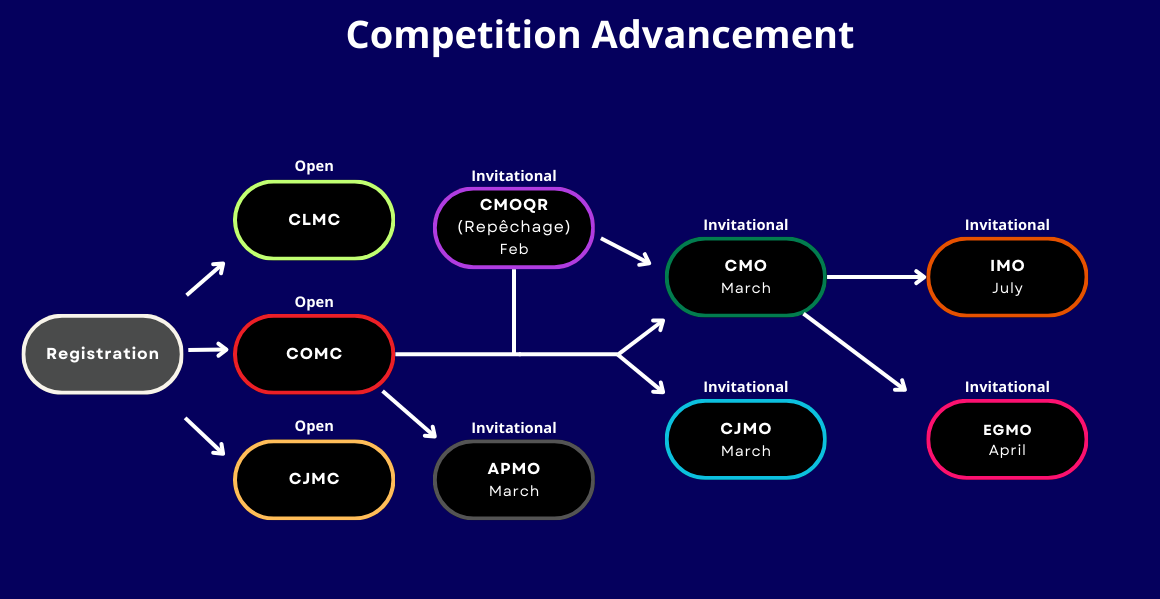
\includegraphics[width=12cm]{./png/Competition-Advancement-EN-V6-Some-Dates-Cropped.png}
\end{center}

\bigbreak
\textbf{Canada Jay Mathematical Competition (CJMC)}

Kỳ thi Toán Canada Jay (CJMC) là một kỳ thi toán của Canada dành cho học sinh từ lớp 8 (lớp cuối của phổ thông cơ sở tại Canada) trở xuống, được sáng lập do các nhà toán học Canada.
Kỳ được đổi tên vào năm 2022 từ tên ban đầu Canadian Mathematical Gray Jay Competition (CMGC) để phù hợp với việc đổi tên của loài chim Canada Jay.
Kỳ thi diễn ra vào tháng 11, sau kỳ thi COMC.

CJMC dài 90 phút, bao gồm 15 câu hỏi trắc nghiệm dựa trên chương trình giảng dạy lớp 5-8, bao gồm 3 nhóm mỗi nhóm gồm 5 câu hỏi với mức độ khó tăng dần từ đầu đến cuối.
Các bài toán mang tính sáng tạo, thú vị tạo một hoạt động mùa thu cho các học sinh và giáo viên để bổ sung cho chương trình giảng dạy toán và xây dựng kỹ năng giải quyết vấn đề của học sinh.
CJMC cung cấp các bài toán hấp dẫn để thảo luận sau cuộc thi và làm cho học sinh có hứng thú với toán.

Một số trường sẽ chọn tham gia Canada Jay bằng cách sử dụng tùy chọn công cụ trực tuyến của CMS.
Thí sinh thi tập trung tại lớp học với giáo viên/giám sát viên bằng máy tính hoặc máy tính bảng Các câu hỏi hiển thị trên màn hình và học sinh chọn câu trả lời của mình.
Ngoài ra, các trường có thể triển khai kỳ thi qua bản in thông thườnh. Các thí sinh đề in sẵn với các câu hỏi và lựa chọn câu trả lời
Các trường sau đó phiếu trả lời của học sinh và tải các bản quét đó lên CMS để chấm điểm và chứng nhận chính thức.

\bigbreak
\textbf{Canada Lynx Mathematical Competition (CLMC)}

Hiệp hội Toán học Canada (CMS) ra mắt cuộc thi toán mới nhất dành cho học sinh lớp 7-12, được thực hiện vào đầu tháng 10.
Mục đích của CLMC thi toán học quốc gia để cung cấp đánh giá sau khi hoàn thành bài kiểm tra để giúp phát triển các kỹ năng toán học của học sinh.
Cuộc thi này được tạo ra để thúc đẩy sự quan tâm đến toán học ở học sinh bất kể trình độ kỹ năng,
để tăng sự tự tin của học sinh vào khả năng toán của cá nhân, cho thấy sự độ hấp dẫn của toán qua góc nhìn khác.

CLMC dài 90 phút, bao gồm 15 câu hỏi trắc nghiệm dựa trên chương trình giảng dạy cốt lõi của lớp 7-11.
Kỳ thi diễn ra vào cuối tháng 9 hoặc đầu tháng 10 hàng năm. Điều này cho phép giáo viên sử dụng CLMC như một công cụ tốt để đánh giá học sinh của họ vào đầu năm học! 
Kỳ thi là cơ hội thử sức cho các học sinh có kỹ năng toán cao, muốn tham gia vào thử thách khó hơn (và thể hiện sự hiểu biết qua việc trình bày lời giải!) để có thể tham dự kỳ thi COMC vào cuối tháng 10.

Ngoài giải thưởng, các thí sinh ở Canada đạt điểm hoàn hảo trong CLMC sẽ được mời tham dự COMC miễn phí.
COMC là cửa ngõ chính để đến với các giải đấu ưu tú chỉ dành cho khách mời, chẳng hạn như Olympic Toán Canada (CMO) và đội tuyển Canada dự Olympic Toán Quốc tế (IMO).

\newpage
\textbf{Canadian Open Mathematics Challenge (COMC)}
Mỗi cuộc thi trong hệ thống CMC đều có cấu trúc và nội dung riêng biệt, phù hợp với trình độ và khả năng của từng lứa tuổi.

COMC là kỳ thi mở cho học sinh ở tất cả các địa điểm, ở tất cả các cấp lớp, trên toàn thế giới.
Để được coi là người tham gia chính thức và do đó đủ điều kiện nhận giải thưởng, sự công nhận hoặc giải thưởng, học sinh và trường học phải đáp ứng các yêu cầu sau:
\begin{itemize}[topsep=0pt, partopsep=0pt, itemsep=0pt]
    \ii Học sinh có quốc tịch Canada hoặc thường trú tại Canada;
    \ii Học sinh phải dưới 19 tuổi tính đến ngày 30 tháng 6 năm trong năm thi;
    \ii Học sinh phải đi học toàn thời gian trực tuyến hoặc trực tiếp ở cả ba cấp tiểu học, trung học cơ sở, Cégep (năm cuối ở tỉnh Quebec) hoặc học tại nhà, kể từ ngày 15 tháng 9 năm trong năm thi;
\end{itemize}

\bigbreak
Việc thi được thực hiện tại bất kỳ địa điểm trên thế giới, chỉ được coi là chính thức nếu được giám sát theo các điều kiện sau:
\begin{itemize}[topsep=0pt, partopsep=0pt, itemsep=0pt]
    \ii Được giám sát trong toàn bộ thời gian thi, tại một trường học hoặc địa điểm cho các điều kiện mà CMS đã phê duyệt cho các kỳ thi được giám sát chính thức.
    \ii Không được phép sử dụng điện thoại di động, máy tính hoặc các thiết bị điện tử khác.
    \ii Thời gian viết 150 phút phải bắt đầu và kết thúc vào khoảng thời gian từ 8 giờ sáng đến 8 giờ tối (0800-2000) theo giờ địa phương vào ngày kiểm tra theo lịch trình
    (Thứ Năm cho tất cả các trường học ở Bắc Mỹ, Nam Mỹ, Trung Mỹ hoặc trong các múi giờ bao gồm các khu vực này; hoặc Thứ Sáu ở những nơi khác trên thế giới).
\end{itemize}

\bigbreak
Đề thi COMC được thiết kế để kiểm tra khả năng tư duy và sáng tạo của học sinh thông qua các câu hỏi về đại số, hình học, tổ hợp và lý thuyết số, thường được chia làm ba phần:
\begin{itemize}[topsep=0pt, partopsep=0pt, itemsep=0pt]
    \ii Phần 1 gồm 4 bài $A1-A4,$ mỗi bài 4 điểm: Các câu hỏi dễ, thường là câu hỏi trắc nghiệm về số học và đại số cơ bản, kiểm tra sự nhạy bén và kỹ năng tư duy logic của học sinh.
    \ii Phần 2 gồm 4 bài $B1-B4,$ mỗi bài 6 điểm: Câu hỏi ở mức trung bình, yêu cầu hiểu biết sâu hơn về tổ hợp và hình học.
    \ii Phần 3 gồm 4 bài $C1-C4,$ mỗi bài 10 điểm: Các câu hỏi khó nhất, đòi hỏi sự sáng tạo và kiến thức mở rộng về lý thuyết số và giải tích.
\end{itemize}

\newpage
\textbf{Giải thưởng dựa trên hiệu suất}

Giải thưởng chỉ được trao cho những học sinh tham gia chính thức, chia thành hai bảng: 
\begin{itemize}[topsep=0pt, partopsep=0pt, itemsep=0pt]
    \ii \textit{Bảng Canada}, chỉ dành cho những học sinh tham gia thi tại Canada (hoặc công dân Canada hoặc thường trú nhân thi ngoài Canada); 
    \ii \textit{Bảng Quốc tế}, chỉ dành cho những người không phải là người Canada thi bên ngoài Canada.
\end{itemize}

\begin{center}
    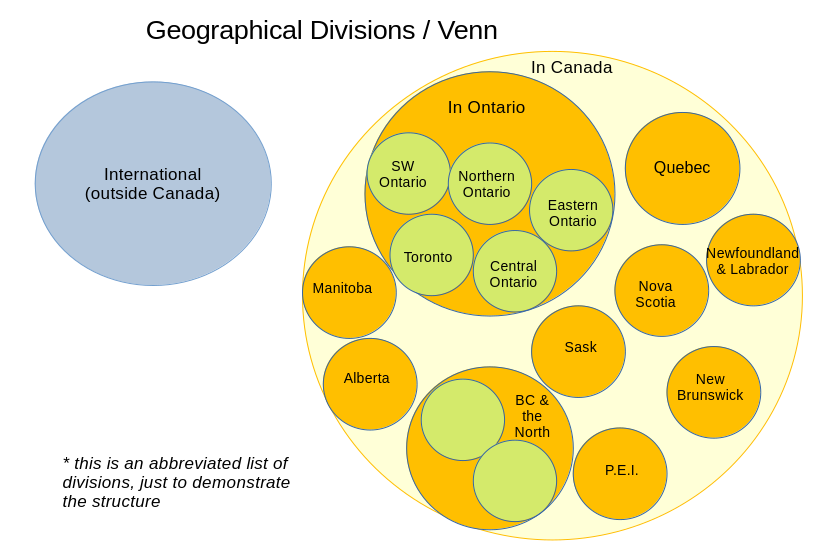
\includegraphics[width=12cm]{./png/divisions-venn-en-2.png}
\end{center}

\textit{Các hạng mục giải thưởng của Bảng Canada:}

Bao gồm các hạng mục giải thưởng cho \textit{Đứng đầu Canada}, \textit{Đứng đầu Tỉnh}, và \textit{Đứng đầu Khu vực}, chia theo mỗi cấp lớp. Sau đây là một số ví dụ:
\begin{itemize}[topsep=0pt, partopsep=0pt, itemsep=0pt]
    \ii \textit{Vô địch Canada}: Toàn thể các thí sinh đều được xét theo hạng mục này. Đây là hạng mục uy giá trị cao nhất;
    \ii \textit{Đứng đầu Canada, Lớp 12 hoặc Cégep}: Dành cho tất cả thí sinh lớp 12 và Cégep;
    \ii \textit{Đứng đầu tỉnh British Columbia}: dành cho tất cả thí sinh (bất kể cấp lớp) ở tỉnh British Columbia;
    \ii \textit{Đứng đầu tỉnh British Columbia, Lớp 10}: dành cho tất cả thí sinh lớp 10 ở tỉnh British Columbia;
\end{itemize}

Sáu điểm thí sinh hàng đầu trong bất kỳ hạng mục nào đều nhận được giải thưởng: Vàng, Bạc, Đồng, và Danh dự.

\begin{remark*}
    Quang Nguyen, thí sinh gốc Việt trong ba năm 2017-2019 dành ba huy chương vàng (khi học lớp 10-12) hạng mục đứng đầu tỉnh New Brunswick, . 
    
    Catherine Doan, thí sinh gốc Việt trong ba năm 2018-2020 dành ba huy chương bạc (khi học lớp 8), đồng (9), vàng (10) trong hạng mục đứng đầu khu vực Đông tỉnh Ontario.
\end{remark*}

\textit{Giải thưởng của Bảng Quốc tế:}

Những thí sinh tham gia chính thức hàng đầu từ bên ngoài Canada, những người không phải là công dân Canada (hoặc thường trú nhân Canada)
được trao giải hạng mục Vô địch Quốc tế, không phụ thuộc cấp lớp.
Ngoài ra, có các hạng mục giải thưởng được chia nhỏ theo cấp lớp, như trong bảng Canada.
Các giải thưởng được trao cho từng hạng mục giải thưởng là Vàng, Bạc, Đồng và Danh dự.

\newpage
\textbf{CMO Qualifying Repêchage (“Repêchage”)}

Sau COMC, các thí sinh chỉ được tham gia khi nhận được thư mời đích danh, phần lớn dựa trên thành tích của sinh viên trong COMC và các cuộc thi từ những năm trước đó.
Để được mời tham gia các cuộc thi của Canada ngoài COMC, thí sinh cần phải là công dân Canada (hoặc thường trú nhân) đang học ở Canada hoặc ở nước ngoài.

Khi kết quả chính thức của COMC được công bố (thường là vào đầu tháng 1), \textit{khoảng} 125 sinh viên đủ điều kiện hàng đầu (tất cả các số liệu đều gần đúng) được chia thành hai nhóm:
\begin{itemize}[topsep=0pt, partopsep=0pt, itemsep=0pt]
    \ii \textit{Khoảng} 50 sinh viên hàng đầu được mời tham dự kỳ thi Olympic Toán học Canada (CMO), đây là kỳ thi hàng đầu cấp quốc gia;
    \ii \textit{Khoảng} 75 sinh viên khác được mời tham gia CMO Qualifying Repêchage (“Repêchage”) vào đầu tháng Hai. Dựa trên kết quả, khoảng 20 thí sinh sẽ được mời tham dự kỳ thi CMO.
\end{itemize}

Repêchage là một bài thi mở làm tại nhà kéo dài một tuần được thực hiện qua email. Đây là một "cơ hội thứ hai" cho một số thí sinh COMC điểm cao nhưng không được mời tham gia CMO.
Các thí sinh này được mời thi Repêchage. Họ nhận 8 bài, tự giải tại nhà, và có một tuần để nộp:
\begin{itemize}[topsep=0pt, partopsep=0pt, itemsep=0pt]
    \ii Phần 1 gồm 6 bài $1-6,$ mỗi bài 10 điểm: Các câu ở mức trung bình, yêu cầu hiểu biết sâu hơn. Độ khó ngang ngửa hoặc cao hơn các bài nhóm $C$ của COMC.
    \ii Phần 2 gồm 2 bài $7-8,$ mỗi bài 20 điểm: Đây là hai bài khó, cách đặt vấn đề không thông dụng đòi hỏi các phương pháp tiếp cận mới, hoặc các lý thuyết bậc cao.
\end{itemize}

\bigbreak
\textbf{Canadian Junior Mathematical Olympiad (CJMO)}

Sau khi kỳ thi Repêchage kết thúc, thông thường tối đa là hai mươi các thí sinh Repêchage kết quả tốt nhưng không được mời tham gia CMO sẽ được mời tham gia CJMO.
Nếu số lượng không đủ, thì những thí sinh COMC có kết quả tốt nhất từ lớp mười trở xuống, không được mời tham gia CMO hoặc Repêchage, sẽ được mời.

Kỳ thi CJMO được thực hiện tại trường (hoặc điểm đăng ký được CMC công nhận) dưới sự giám sát của giáo viên hoặc giám khảo do CMC quy định.

CJMO thi trong ba giờ với năm bài, thường được tổ chức cùng lúc vào cuối tháng Ba.
Độ khó của các bài thi CJMO là tương đương với kỳ thi CMO, nhưng không đòi hỏi các công cụ toán nhưng năm cuối trung học để giải quyết.

Các thí sinh cạnh tranh danh hiệu chính là \textit{Vô địch CJMO} và được trao huy chương vàng. Các thí sinh còn lại, tuỳ theo kết quả, được trao huy chương Bạc, Đồng và Danh dự.
Thông thường, CJMO có không quá 4 giải thường.

\newpage
\textbf{Canadian Mathematical Olympiad (CMO)}

CMO là kỳ thi dành cho khoảng 50 thí sinh qua vòng thi COMC và 20 từ vòng thi Repêchage. Thí sinh giải năm bài trong vòng ba giờ.
Kỳ thi thường được tổ chức vào cuối tháng Ba cùng lúc với CJMO.

CMO là kỳ thi quan trọng nhất dành cho những thí sinh muốn giành được một vị trí trong Đội tuyển Toán Canada (Math Team Canada - MTC),
đây là nhóm thí sinh sẽ được chọn để đại diện cho Canada tại Olympic Toán Quốc tế (IMO) vào mùa hè. 
Các kỳ thi CMO đều được thực hiện tại trường (hoặc điểm đăng ký được CMC công nhận) dưới sự giám sát của giáo viên hoặc giám khảo do CMC quy định.

Các thí sinh cạnh tranh danh hiệu chính là \textit{Vô địch CMO} và được trao huy chương vàng. Các thí sinh còn lại, tuỳ theo kết quả, được trao huy chương Bạc, Đồng và Danh dự.
Thông thường, CMO có không quá 6 giải thường.

Cúp vô địch CMO là một chiếc cúp kích thước đầy đủ để tưởng nhớ vĩnh viễn các nhà vô địch. 
Chiếc cúp thường được cho mượn đến trường của nhà Vô địch CMO để trưng bày trong một năm.

\begin{center}
    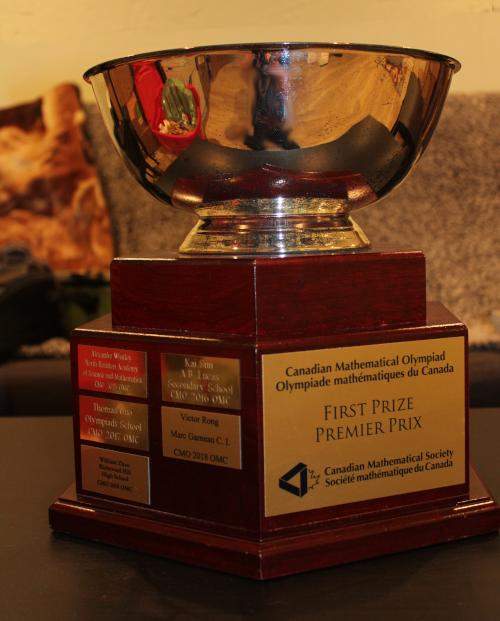
\includegraphics[width=5cm]{./png/cmo-trophy-2022.png}
\end{center}

Mỗi năm, một số tiền được lập ngân sách trước được phân bổ từ Hiệp hội Toán học Canada và các thành viên và nhà tài trợ của nó.
Thông thường, giải thưởng này được chia nhỏ để đảm bảo người giành huy chương vàng CMO nhận được 2000 đô la Canada (trừ khi có các thí sinh đồng hạng),
và Bạc, Đồng và Danh dự cũng nhận được tiền thưởng với số tiền giảm dần cho mỗi người. CJMO cũng tương tự nhưng với các giải thưởng tiền mặt nhỏ hơn đáng kể.

\begin{remark*}
    Minh Tue Vo, thí sinh gốc Việt, hai lần đứng đầu kỳ thi CMO, trong hai năm 1984-1985.
\end{remark*}

\textit{Giải thưởng Matthew Brenan cho lời giải hay nhất:}

Vào năm 2021, CMS và cộng đồng toán học đã mất đi một trong những thành viên có giá trị nhất.
Matthew đại diện cho Canada hai lần tại Olympic Toán Quốc tế, giành huy chương đồng vào năm 2011 và huy chương vàng vào năm 2012.
Ông trở lại IMO với tư cách là phó quan sát viên lãnh đạo vào năm 2014 và 2017, và là lãnh đạo vào năm 2019.
Matt đam mê toán Olympic và đã phục vụ trong ủy ban Olympic Toán Canada từ năm 2014.
Anh ấy cũng đã đóng góp rất nhiều vào việc tạo ra và lựa chọn vấn đề.

Để vinh danh Matthew, CMS đã tạo ra Giải thưởng Matthew Brennan cho Giải pháp CMO tốt nhất.
Giải được trao hàng năm cho (các) thí sinh viên có lời giải tốt nhất cho duy nhất một bài của CMO của năm đó.
Lời giải họ sẽ được đưa vào các lời giải chính thức và thí sinh sẽ nhận được giải thưởng bằng tiền.

\textit{Giải thưởng tri ân giáo viên:}

Để ghi nhận những đóng góp có giá trị của giáo viên trong việc tạo điều kiện cho học sinh COMC tham gia,
một số giáo viên ở Canada sẽ đủ điều kiện nhận một số lượng các giải thưởng từ Maplesoft và từ Hiệp hội Toán học Canada vào tháng Giêng.

\bigbreak
\textbf{Olympic Toán Nữ Châu Âu (EGMO) và Olympic Toán Châu Á-Thái Bình Dương (APMO)}

Vào đầu tháng Ba, Hiệp hội Toán học Canada cũng mời 20-30 thí sinh kết quả tốt nhất tại COMC đại diện cho Canada tham dự Olympic Toán Châu Á-Thái Bình Dương (APMO).
APMO được tiến hành như kỳ thi như CMO, tại trong trường học của thí sinh dưới sự giám sát của giáo viên.

APMO được tổ chức vào chiều thứ Hai thứ hai của tháng Ba đối với các quốc gia tham gia ở Bắc và Nam Mỹ, và vào sáng thứ Ba thứ hai của tháng Ba đối với các quốc gia tham gia ở Tây Thái Bình Dương và Châu Á.
Cuộc thi APMO bao gồm một bài báo dài bốn giờ bao gồm năm câu hỏi có độ khó khác nhau và mỗi câu hỏi có số điểm tối đa là 7 điểm.
Tất cả các thí sinh APMO sẽ nhận được Giấy chứng nhận Giải thưởng, Danh dự hoặc Đại diện.

Hiệp hội Toán học Canada mời bốn nữ thí sinh xuất sắc nhất của các kỳ thi CMO, CJMO, COMC vào đội tuyến toán Canada để gửi đến Châu Âu tham dự kỳ thi Olympic Toán Nữ Châu Âu (EGMO) vào tháng Tư.

\bigbreak
\textbf{Lựa chọn Đội tuyển Canada đi dự IMO}

Đội tuyển Canada tại IMO được lựa chọn theo quy trình sau:

\begin{center}
    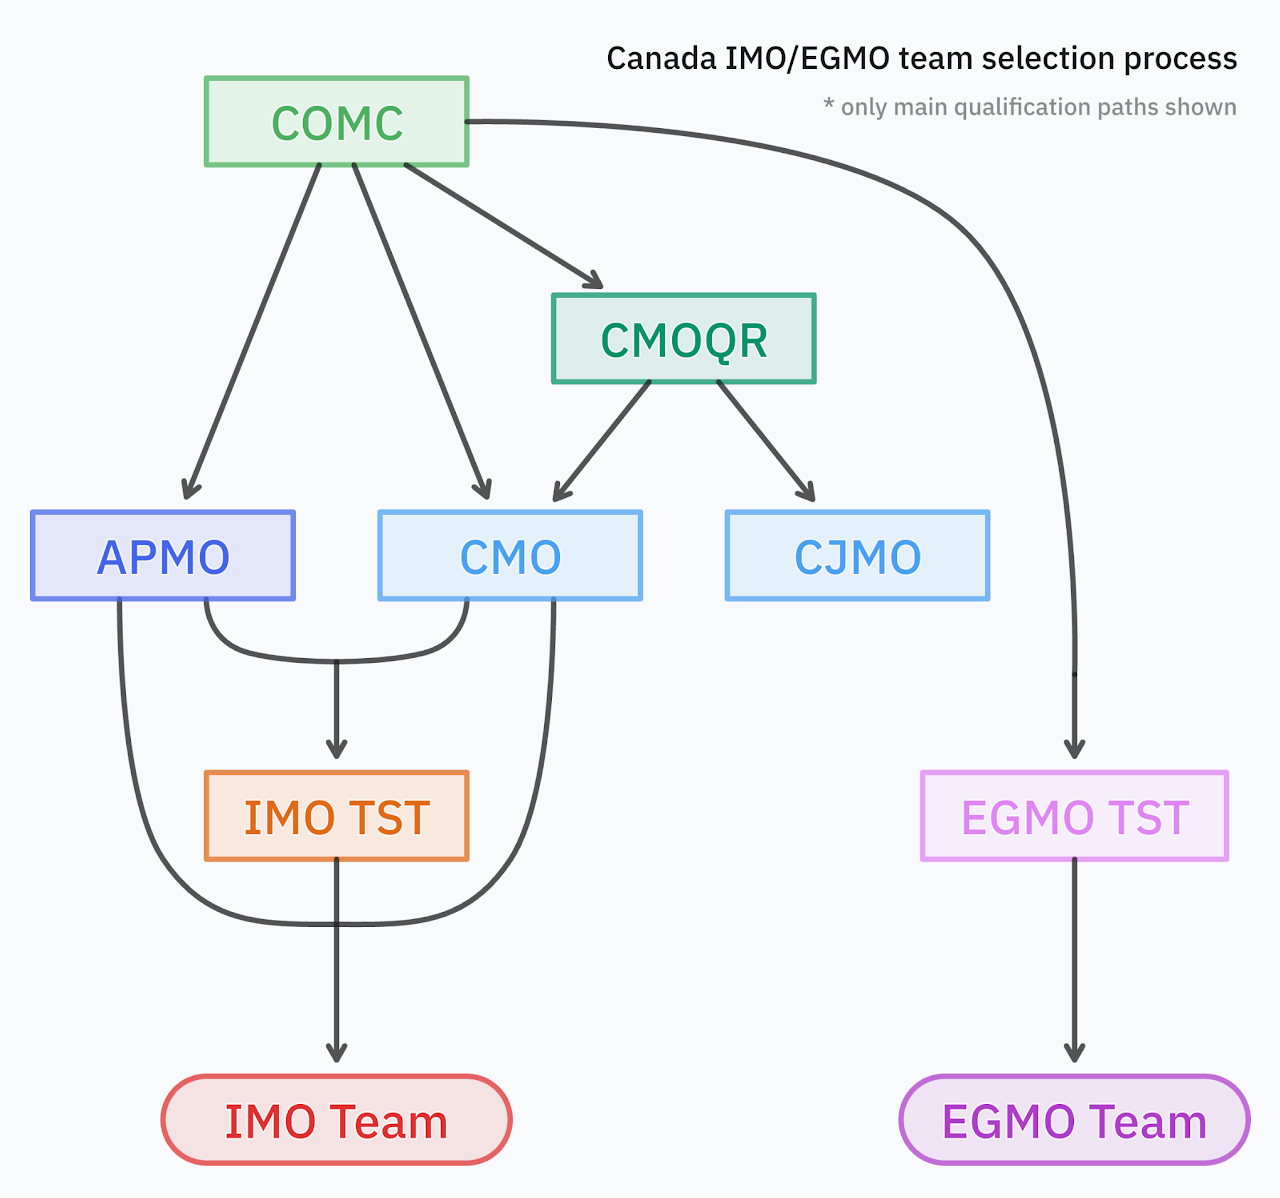
\includegraphics[width=6cm]{./png/Canadian IMO EGMO selection process.png}
\end{center}

\begin{itemize}[topsep=0pt, partopsep=0pt, itemsep=0pt]
    \ii Vòng đầu tiên: là kỳ thi COMC. Kỳ thi này dành cho tất cả mọi thí sinh và thường diễn ra vào cuối tháng Mười. Bất cứ thí sinh nào muốn có đủ điều kiện tham gia IMO đều phải bắt đầu từ COMC.
    \ii Các vòng Olympic:
    \begin{itemize}[topsep=0pt, partopsep=0pt, itemsep=0pt]
        \ii Olympic Toán Châu Á Thái Bình Dương (APMO): Những sinh viên đạt điểm cao trong COMC được mời tham gia APMO. Khoảng 30 sinh viên được mời. Kỳ thi vào thứ Hai thứ hai của tháng Ba.
        \ii Olympic Toán Canada (CMO): 50 thí sinh hàng đầu COMC được mời trực tiếp đến CMO. Nhóm tiếp theo gồm 75 sinh viên viết COMC Repêchage, từ đó 20-30 sinh viên khác được mời. Kỳ thi vào vào đầu tháng Ba.
    \end{itemize}
    \textit{Các học sinh được mời tham gia Trại Mùa đông CMS là đảm bảo đủ điều kiện cho cả APMO và CMO.}
    \ii Vòng chung kết: Bài thi chọn Đội tuyển IMO của Canada (Team Selection Test - TST):
    Dựa trên kết quả của APMO và CMO, một nhóm sinh viên sẽ được mời viết bài thi chọn cuối cùng, diễn ra vào giữa tháng Tư.
    \ii Đội tuyển IMO sẽ được lựa chọn dựa trên kết quả của cả ba kỳ CMO, APMO và TST gần nhất.
\end{itemize}

\newpage
\textbf{Tập trung luyện thi}

\textit{Trại mùa đông}: Trại mùa đông chỉ dành cho những thí sinh hàng đầu diễn ra vào đầu tháng 1 tại Toronto, thường là tại Đại học York.

\textit{Trại mùa hè}: Trạm Nghiên cứu Quốc tế Banff về Đổi mới và Khám phá Toán học (BIRS) là một liên doanh hợp tác Canada-Mỹ-Mexico cung cấp môi trường cho sự tương tác sáng tạo cũng như trao đổi ý tưởng,
kiến thức và phương pháp trong Khoa học Toán học, với các ngành liên quan và với ngành công nghiệp.
Trạm nghiên cứu được đặt tại Trung tâm Banff ở Alberta và được hỗ trợ bởi Hội đồng Nghiên cứu Khoa học Tự nhiên và Kỹ thuật của Canada (NSERC), Hoa Kỳ,
Quỹ Khoa học Quốc gia (NSF) và Giáo dục và Công nghệ Tiên tiến của Alberta.

Sáu học sinh được tuyển chọn tập trung tại BIRS trong thời gian khoảng 2 tuần trước kỳ thi IMO. 

\textit{Các trại mùa hè khác:} Khoảng 24 học sinh từ lớp 10 trở xuống có thành tích tốt tại kỳ thi COMC sẽ được mời tham gia \textit{Trại Toán mùa hè CMS Canada } do Đại học Toronto tổ chức.
Những học sinh thể hiện thành tích cao ở cấp lớp trong khu vực hoặc tỉnh của họ và được đề cử có thể được mời tham gia \textit{Trại Toán mùa hè Khu vực}
được tổ chức với sự hợp tác của đối tác đại học CMS trong tỉnh.

\bigbreak
\textbf{Đội tuyển Canada tại IMO}

\begin{itemize}[topsep=0pt, partopsep=0pt, itemsep=0pt]
    \ii Ba kỳ xếp hạng cao nhất (thứ 5): 2012 (3 vàng 1 bạc 2 đồng), 2021 (3 vàng 3 bạc), 2023 (1 vàng 4 bạc 1 đồng), trong đó năm 2023 cũng là năm có điểm cao nhất (183).
    \ii 1 học sinh tham dự 6 kỳ (Zhuo Qun (Alex) Song), 1 học sinh tham dự 5 kỳ (Thomas Guo), bốn học sinh tham dự 4 kỳ, 16 học sinh tham dự 3 kỳ IMO.
\end{itemize}

\bigbreak
\textbf{Các gương mặt đáng chú ý}

\textbf{Zhuo Qun (Alex) Song}: sinh ra ở Thiên Tân, Trung Quốc vào năm 1997. Cha mẹ anh di cư đến Canada vào năm 2002 và định cư tại Waterloo, ON.
AnAlexh quan tâm đến toán từ khi còn nhỏ; và bắt đầu tham gia các cuộc thi ở Lớp 1, rồi tham gia Cuộc thi Pythagoras, dành cho học sinh lớp 6.
Khi khám phá ra sở thích của mình đối với toán, Alex tham dư các cuộc thi khác nhau ở các cấp độ khác nhau, bao gồm COMC (Canada) và AMC-10 (Hoa Kỳ) khi học Lớp 4.

Sau khi tham gia USAMO (Olympic Toán học Hoa Kỳ) ở lớp 4, Alex bắt đầu quan tâm đến các bài toán Olympiad, nhất là giải các bài khó khăn thú vị.
Năm lớp 7, Alex đã tham gia Trại mùa đông CMS 2010, một trại huấn luyện để xác định 6 thành viên của Đội IMO (Olympic Toán Quốc tế) Canada trong số 12 ứng cử viên hàng đầu.
Alex rất thích trại đầu tiên của mình vì đây là lần đầu tiên, cậu chỉ làm mỗi toán trong một thời gian dài.
Alex nhận giải khuyến khích thi APMO và vị trí số 1 trong CMO (Olympic Toán học Canada) trên đường tham dự đến Olympic Toán Quốc tế và dành chiếc huy chương đồng đầu tiên năm 13 tuổi.

Alex ấy đã chuyển từ Canada đến Mỹ để theo học Học viện Phillips Exeter vào năm 2011. Alex được trao huy chương vàng trong APMO, một giải khuyến khích USAMO và vị trí thứ 3 trong CMO khi học lớp 8.
Kết quả này giúp Alex lần thứ hai đã lọt vào đội IMO Canada lần thứ hai, và chiếc huy chương vàng IMO đầu tiên của mình.
Trong những năm tiếp theo, Alex đã liên tục giành được thêm 4 huy chương vàng với đội Canada trong IMO, trở thành người duy nhất được 5 huy chương vàng trong lịch sử Olympic Toán Quốc tế,
trong đó có một huy chương vàng tuyệt đối 42 điểm vào năm 2015.

Alex học toán tại Đại học Princeton, rồi Đại học Illinois Urbana-Champaign, và bắt đầu làm việc bán thời gian về đính toán định lượng (cho đầu tư tài chính) tại Citadel LLC.
Bên cạnh toán, Alex thích chơi piano, chơi cờ vua, bài bridge, quay Rubik, và các trò chơi tư duy. Anh ấy quan tâm đến khoa học, đặc biệt là vật lý và hóa học.

\textbf{Alexander Whatley}: Ba lần tham dự IMO 2013-2015, ba huy chương đồng, mỗi lần anh thiếu đúng một điểm để được huy chương bạc.
Hiện nay anh nghiên cứu về bộ vi xử lý thần kính (neuromorphic processors), mô phỏng tính toán não tại đại học Cornell.

\textbf{Minh-Tue Vo}: Thí sinh gốc Việt, hai lần tham dự IMO 1984-1985, huy chương bạc 1985. Hiện anh là Phó chủ tịch, Bank of America, chuyên phụ trách các dự án sát nhập doanh nghiệp.

\end{otherlanguage*}

\end{document}